\section{Understanding Boosting and ICA}


\subsection{Adaboost}

The figure below shows a data set that contains two classes ('+' and 'o'). The instances are labeled A-E.

\begin{center}
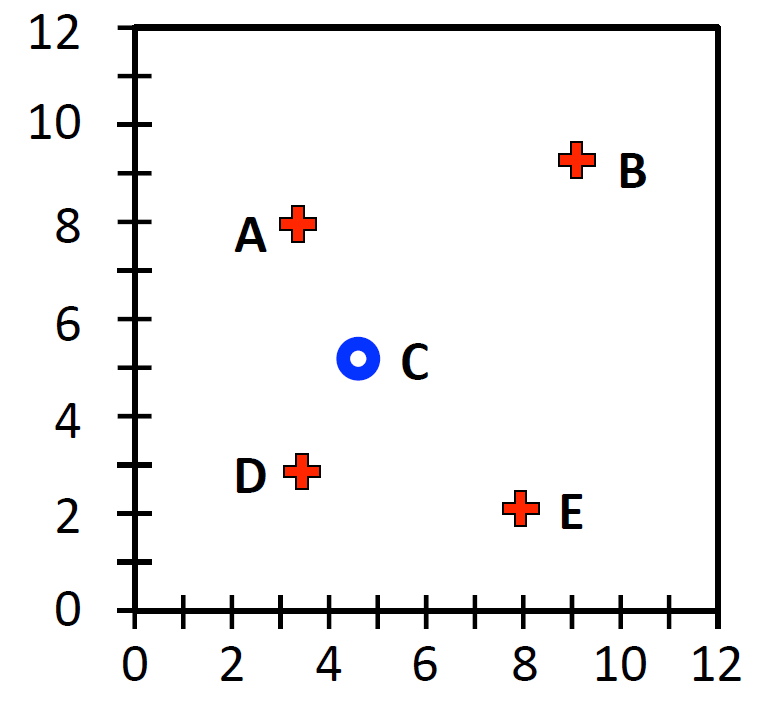
\includegraphics[trim={0cm 0 0 0},clip,scale=0.4]{figs/fig1.png}
\end{center}

If we train Adaboost to solve the classification problem.

\begin{enumerate}
    \item Which instances will have their weights increased at the end of the first boosting iteration? (Explain)
    \item What is the \textbf{minimum} number of iterations that the algorithm could take to achieve zero training error? (Explain)
    \item Is it possible to add another example to the data set to guarantee that boosting achieves zero training error in just two iterations? If so, how? If not, why?
\end{enumerate}

\subsection{Affine Transformation of Random variables}
Let ${\bf X}$ be a $d$-dimensional random vector with mean ${\bf \mu}$ and covariance matrix  $\Sigma$. Let ${\bf Y} = A{\bf X} + {\bf b}$, where $A$ is a $n \times d$ matrix and ${\bf b}$ is a $n$-dimensional vector.

\begin{enumerate}
    \item Show that the mean of ${\bf Y}$ is $A {\bf \mu } + {\bf b}$
    \item Show that the covariance matrix ${\bf Y}$ is $A \Sigma A^\top$
\end{enumerate}

\subsection{Difference between Correlation and Independence}

Consider the discrete random variable $X$ described as follows
$$ \mathbb{P}(X = i ) = \left\{ \begin{array}{ll} 1/3 & \text{ if } i = -1\\
1/3 & \text{ if } i = 0\\
1/3 & \text{ if } i = 1\end{array}\right.$$
We also define the random variable $Y = 1 - X^2$.

\begin{enumerate}
    \item Compute the values of $\mathbb{E}(X)$ and $\mathbb{E}(Y)$.
    \item Compute $\mathbb{E}(XY)$ and $Cov(X,Y)$. Are $X$ and $Y$ uncorrelated?
    \item Are $X$ and $Y$ independent? i.e., $\mathbb{P}(X = i\, , \, Y=j) = \mathbb{P}(X = i) \mathbb{P}(Y =j)$?
\end{enumerate}





